\chapter{Anforderungsanalyse}\label{chap:requirements}

\section{Produktüberblick}
Um die Anforderungen erstellen und verstehen zu können muss zunächst einmal der Ausganszustand, also der jetzige Desktopclient des \nameformat{\gls{crm}} (Eigenschreibweise für das \gls{CRM} Produkt der Firma \nameformat{combit GmbH}) betrachtet werden. Wie am Begriff \gls{CRM} bereits zu erkennen handelt es sich dabei um ein Programm das der Verwaltung und Vernetzung von Kunden- und Kontaktdaten dient. Neben den typischen Einsatzbereichen von \gls{CRM}-Produkten wie die erwähnte Verwaltung von Kundendaten, Terminen und Aufgaben legt die combit GmbH allerdings viel Wert darauf, das Programm möglichst flexibel zu gestalten und damit viele weitere Einsatzbereiche von einer großen Anzahl verschiedener Kundengruppen zu ermöglichen. Einige Beispiele hierfür sind die mitgelieferten, fertigen Lösungen (im Kontext des \nameformat{\gls{crm}} ``Solutions'' genannt) mit denen unter anderem Immobilien gehandhabt, die Vermittlung von Arbeitsstellen an Drittfirmen organisiert oder ein Ticket-System aufgebaut werden können. Zudem ist eine Musterlösung für den \gls{dsgvo}-konformen Umgang mit all diesen Daten integriert. Unabhängig von diesen Lösungen stehen gewisse Funktionalitäten die jedoch auf den Daten einer Lösung aufbauen --- Import und Export von Daten in viele verschiedene Formate, Versand von (Serien-) E-Mails oder etwa die Generierung von Berichten (Reports) durch ein zweites internes Produkt ``List \& Label'' --- immer zur Verfügung.
Eine Solution stellt die grundsätzliche Organisation der Daten in bestimmte Bereiche oder Szenarien dar und kann von jeder Firma individuell konfiguriert werden. Jede Solution ist durch eine Menge von Datenbanktabellen und darauf basierenden Ansichten zur Visualisierung der in den Tabellen enthaltenen Entitäten und Relationen definiert. Anhand der in Abbildung~\ref{fig:crm_ui} gezeigten Standard-Solution  ``Large''  ist links eine Liste der verfügbaren Ansichten und rechts die Detailansicht einer Entität der ``Firmen''-Ansicht zu sehen. Außerdem wird hier auch die allgemeine Trennung zwischen Haupt-UI und ansichtsspezifischer UI ersichtlich. Anstelle der Detailansicht kann auch eine Listenansicht (tabellenförmige Auflistung aller Entitäten), eine Berichtsansicht, eine Webansicht (momentan mithilfe des Internet Explorer realisiert) und eine Kombinationsansicht, bei der sowohl die Übersichtsliste als auch die Details sichtbar sind, angezeigt werden.

\begin{figure}
    \centering
    \captionsetup{justification=centering}
    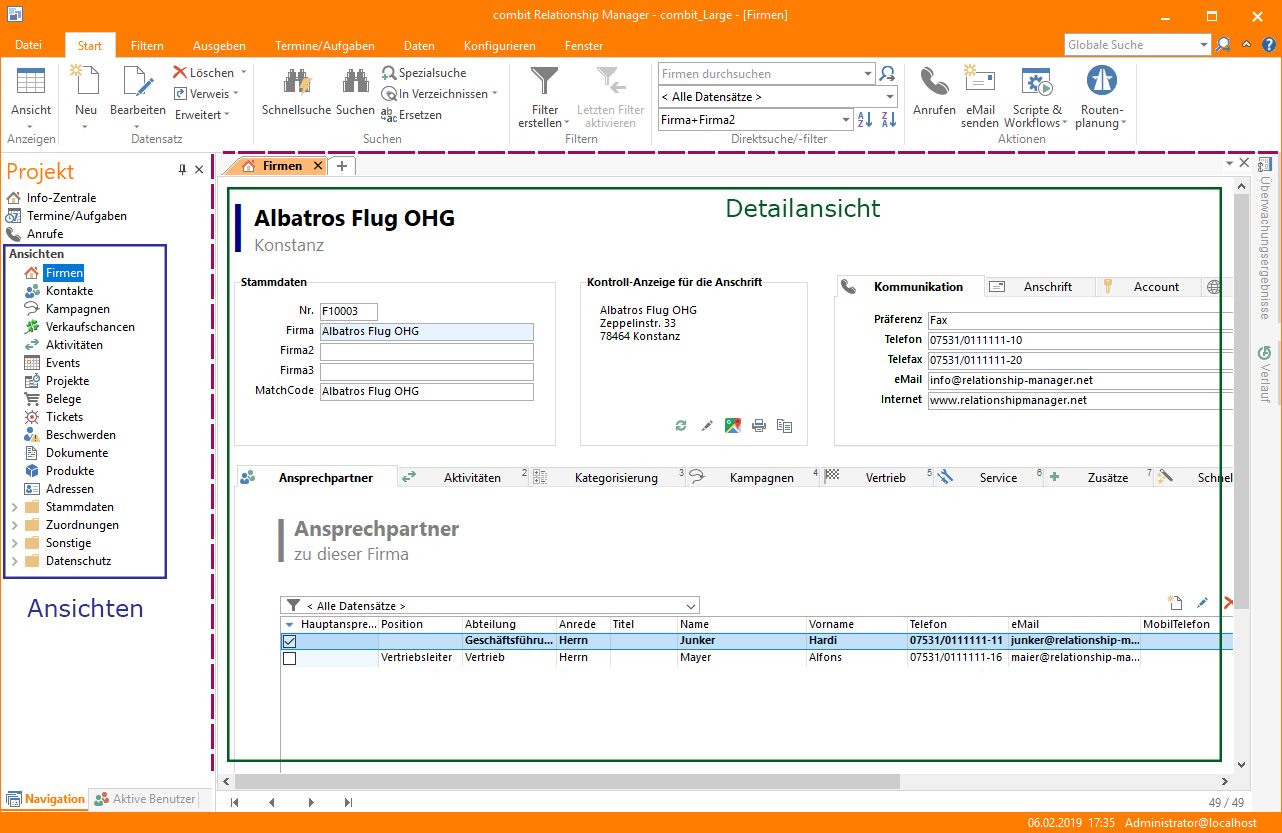
\includegraphics[width=\textwidth]{figures/crm_ui.png}
        \caption{Grafische Oberfläche des \gls{crm} Desktopclient}\label{fig:crm_ui}
\end{figure}

Aus technischer Sicht ist der \gls{crm} in drei Schichten getrennt. Die zu verwaltenden Daten werden entweder in einer Microsoft SQL Server- oder einer PostgreSQL-Datenbank gespeichert. Eine Besonderheit hierbei ist die Tatsache dass Relationen zwischen Datenbanktabellen nicht durch Fremdschlüssel und zugehörige auf Datenbankebene sondern durch virtuelle Relationen zwischen Ansichten im C++-Kern der Anwendung, realisiert sind. Dies erlaubt einen flexibleren Umgang mit diesen und vereinfacht das Ändern von Datenbanktabelle, Ansichten und Relationen direkt aus der Oberfläche des \nameformat{\gls{crm}}.
Der \nameformat{\gls{crm}}-Core bildet die zweite Schicht und ist für den Datenbankzugriff und die Business Logic \fixme{footnote} verantwortlich. Diese beiden Schichten sollen von der Erstellung der neuen Weboberfläche möglichst unberührt bleiben. Einzig die API-Anbindung für die UI muss an dieser Stelle integriert werden --- betrachtet wird die API in dieser Arbeit jedoch nur aus Sicht der Oberfläche, die Integration im Backend findet zu einem späteren Zeitpunkt statt.
Aufsetzend auf dem Kern existieren parallel der Desktopclient, ebenfalls in C++ geschrieben, der WebAccess für Desktopbrowser und der WebAccess Mobile für mobile Endgeräte. Zwischen Core und Webaccess (Mobile) gibt es noch einen mit ASP.NET \fixme{footnote?} realisierten .NET-Wrapper, welcher den Zugriff auf Daten per HTTP ermöglicht.

Abbildung~\ref{fig:crm_technical_stack} zeigt eine Übersicht der momentanen Architektur, Abbildung~\ref{fig:crm_future_technical_stack} hingegen, wie die Architektur in Zukunft aufgebaut sein könnte.

\begin{figure}
    \centering
    \captionsetup{justification=centering}
    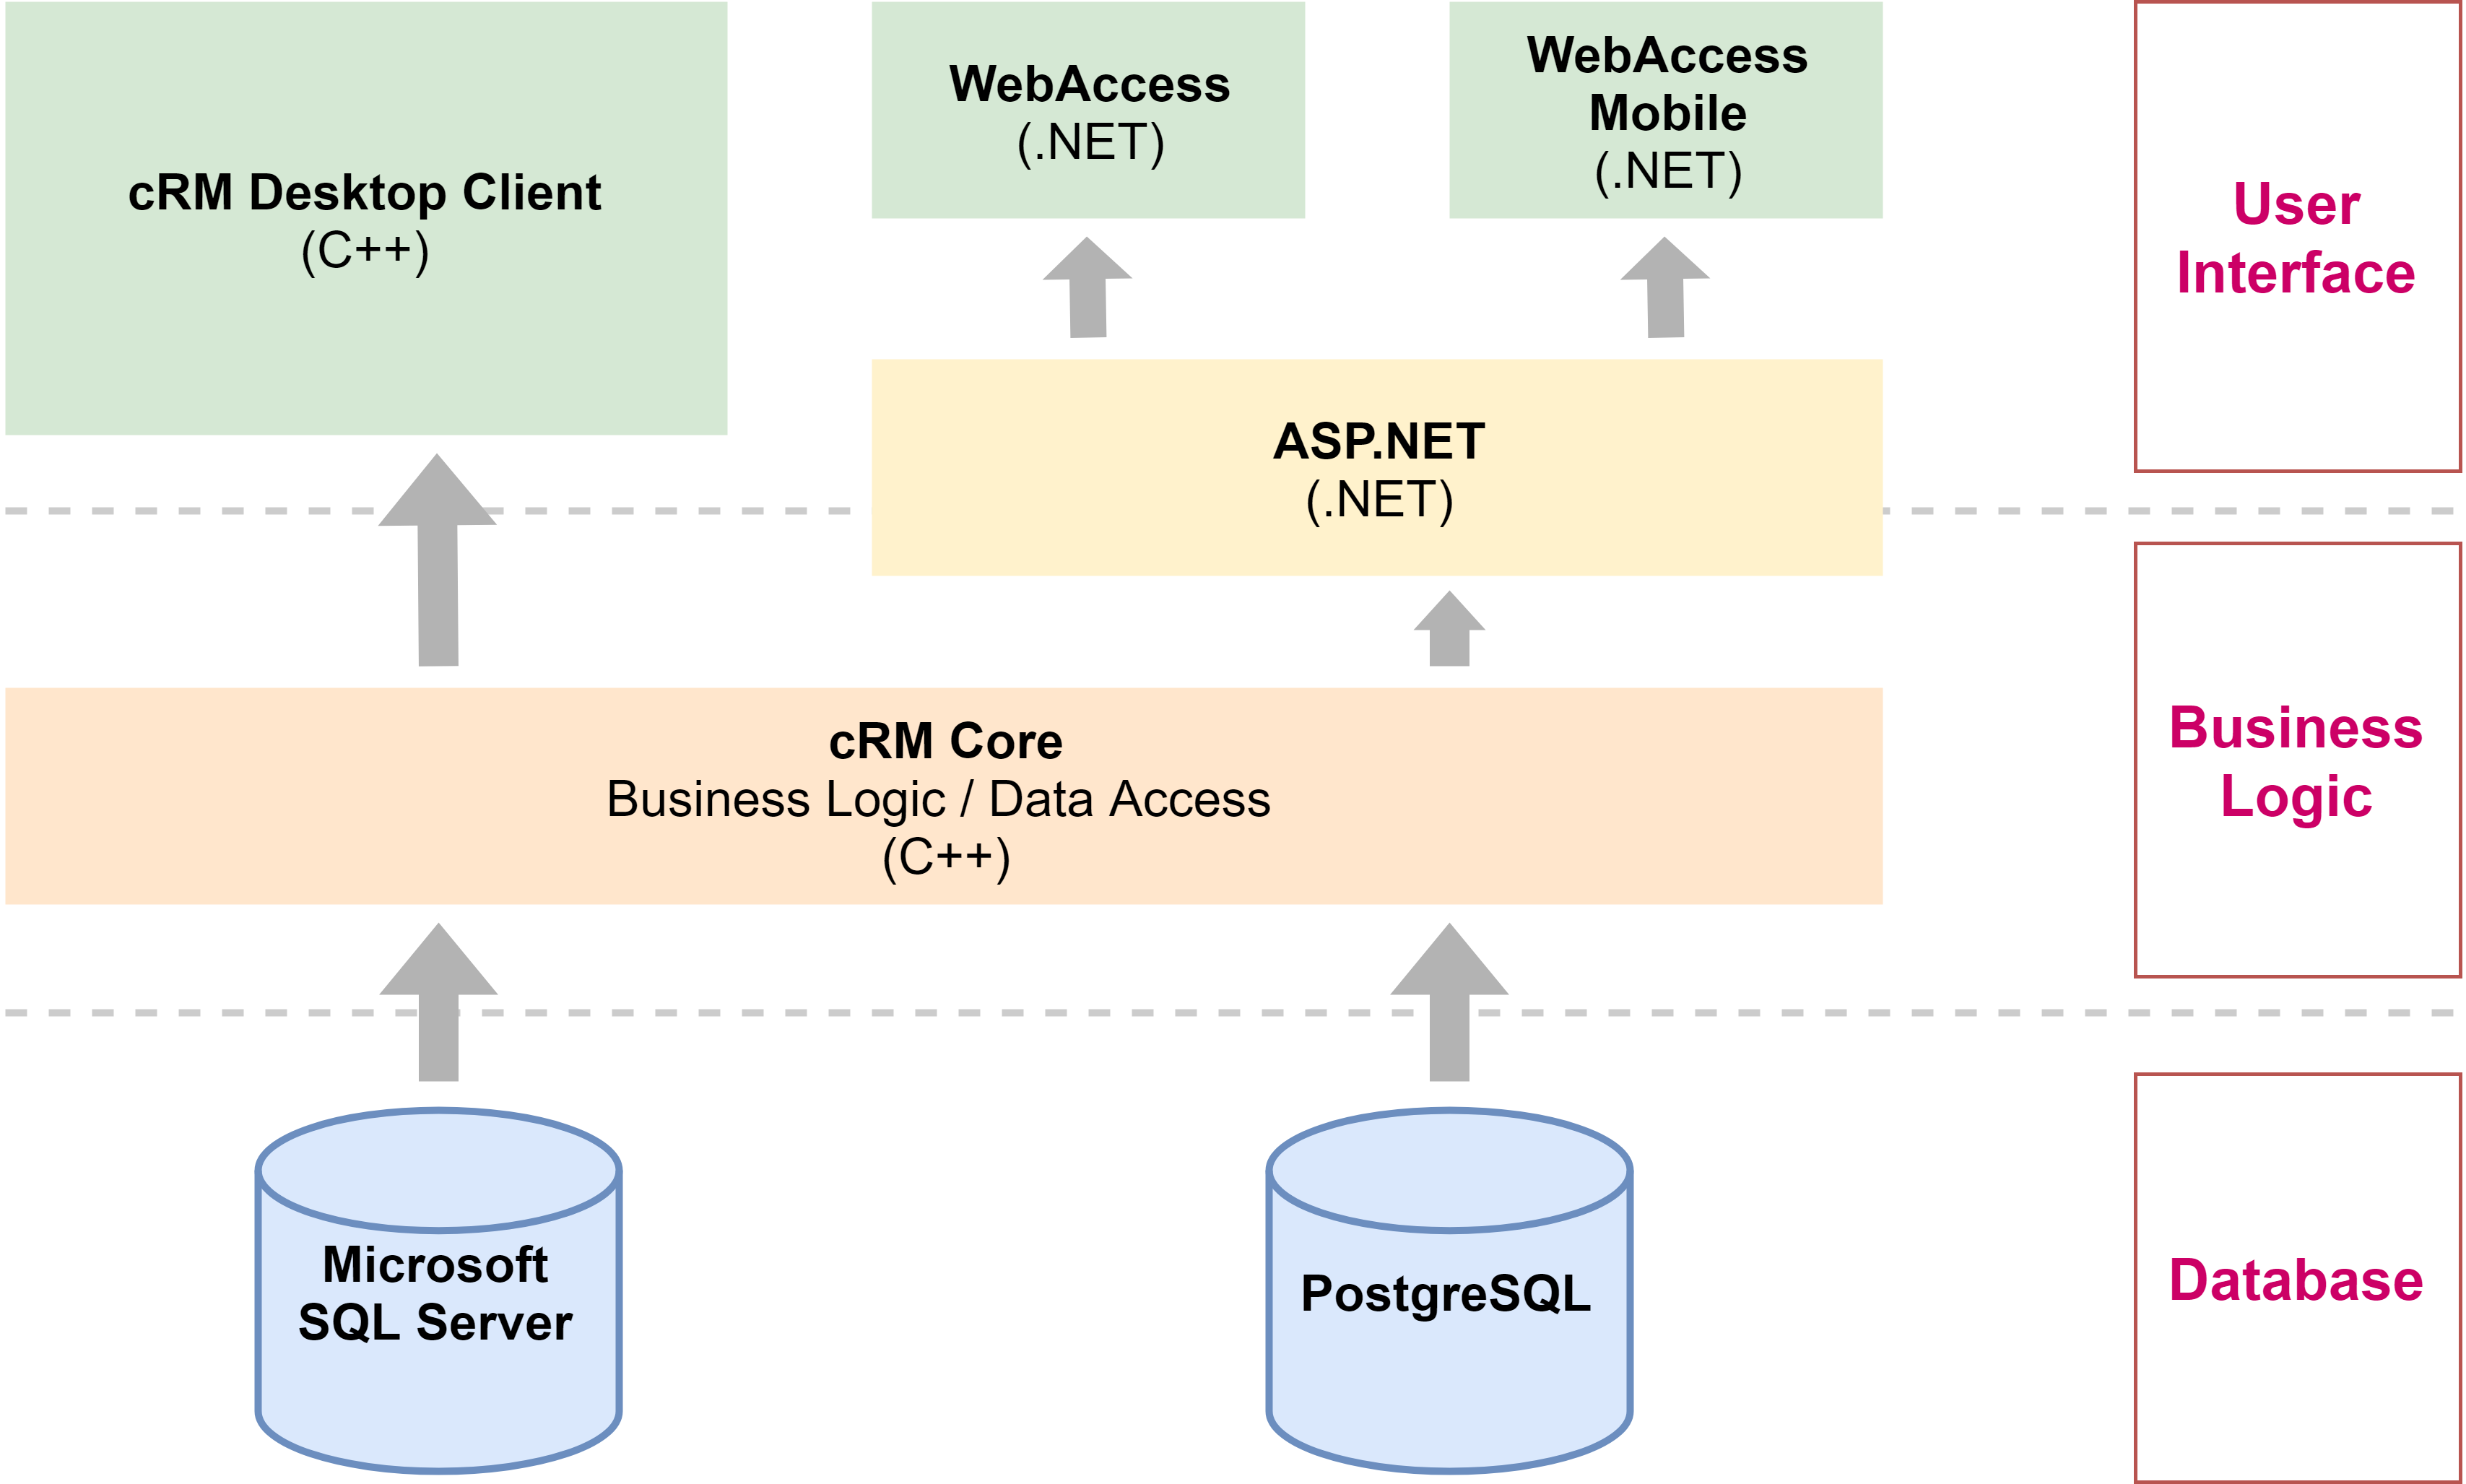
\includegraphics[width=\textwidth]{figures/crm_technical_stack.png}
        \caption{Aktueller technischer Aufbau des \gls{crm}}\label{fig:crm_technical_stack}
\end{figure}

\begin{figure}
    \centering
    \captionsetup{justification=centering}
    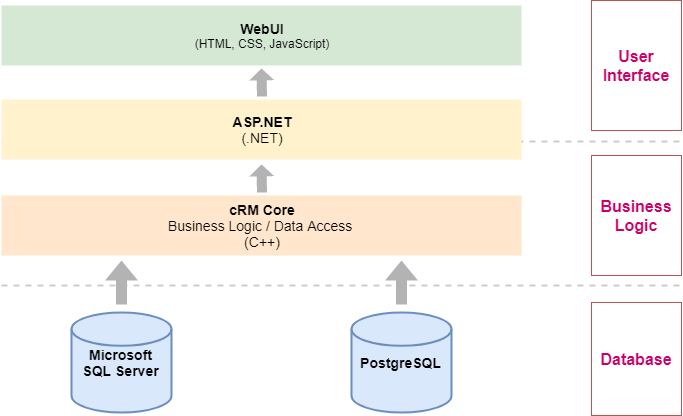
\includegraphics[width=\textwidth]{figures/crm_future_technical_stack.png}
        \caption{Möglicher zukünftiger technischer Aufbau des \gls{crm}}\label{fig:crm_future_technical_stack}
\end{figure}


\section{Funktionale Anforderungen}
In diesem Teil des Kapitels werden funktionale Anforderungen welche die Web-UI unterstützen soll aufgelistet und kurz erläutert.

\subsection{\acrlong{crm}}
\subsubsection{Automatisierte Erstellung}
Die meisten Kunden haben entweder bereits ihre eigenen Ansichten erstellt oder benutzen angepasste Versionen der mitgelieferten Designs. Wenn das Ziel ist, langfristig die komplette UI-Schicht ins Web zu überführen muss dieser Prozess für die Benutzer leicht und zugänglich genug sein um nicht schon im Voraus abgelehnt zu werden. Es ist daher unumgänglich dass alle bisherigen Ansichten mit minimalem Aufwand seitens deren Nutzer im Web weiterverwendet werden können. Einige kleine Anpassungen sind tolerierbar, jede Ansicht neu zu erstellen jedoch nicht. Eines der Hauptziele dieser Arbeit ist es daher eine automatische Umwandlung bestehender Ansichten zu ermöglichen --- hierfür muss die aktuelle UI-Spezifikation analysiert und eine neue Spezifikation erstellt werden, welche Implementierungen aus der vorherigen generieren kann.

\subsubsection{Benutzerverwaltung}
Die Benutzer und deren Rechte werden vollständig im Backend verwaltet. Es muss allerdings bei der Umsetzung der Konfigurationsoberfläche und bei der Umsetzung der Rechte besonders sorgfältig geprüft werden, ob weiterhin der volle Funktionsumfang gewährleistet ist. Sollten bestimmte Rechte für Benutzer oder Gruppen nicht mehr anpassbar sein  oder fehlerhaft angewendet werden ist unter Umständen der komplette \nameformat{\gls{crm}} nicht mehr vernünftig nutzbar.

\subsubsection{Edit-Modus}
Änderungen in der Detailansicht werden nicht direkt an die Datenbank übertragen, sondern nur als geändert markiert. Der Benutzer hat dann die Möglichkeit diese zu verwerfen oder den entsprechenden Datensatz zu speichern und die Informationen in die Datenbank zu schreiben.

\subsubsection{Individualisierung}
Die Individualisierung der beiden Hauptansichten für Datenentitäten, die Detail- und Listenansicht, ist zur effektiven Visualisierung bestimmter Sachverhältnisse ausschlaggebend. Bei der Listenansicht können beispielsweise Datenbankspalten ein- bzw.\ ausgeblendet und frei angeordnet werden, Spalten je nach Datentyp formatiert und spezielle Werte nach selbst definierten Regeln hervorgehoben werden. Die Detailansicht ist noch mächtiger, hier kann jedes UI-Element frei platziert werden, mit Sichtbarkeits- und Formatierungsbedingungen versehen und mit anderen Feldern verknüpft werden (Änderung in Feld A löst Änderung in Feld B aus). Um diese Einstellungen vorzunehmen existiert ein kompletter Eingabemaskendesigner welcher dem Benutzer per \gls{wysiwyg}-Prinzip \fixme{footnote?} das Designen erleichtert.
Die Weboberfläche sollte diese Funktionalität möglichst vollständig abbilden.

\subsubsection{Berichts- und Webansicht}
Wie in der Übersicht erklärt werden Berichte von einem zweiten Produkt der Firma \nameformat{combit GmbH}, \nameformat{\gls{ll}}, gehandhabt. Dieses besitzt bereits zum jetzigen Zeitpunkt einen entsprechende Weboberfläche die zukünftig für die Erstellung und das Anzeigen von Berichten genutzt werden kann. 
Auch die Webansicht kann weiterhin unterstützt werden indem darin anzuzeigende Ressourcen in ein iframe-Tag \fixme{footnote?} eingebettet werden.

\subsubsection{Suche / Filter / Sortierung}
Suchen und Filter von Datensätzen können weiterhin mit bestehenden Techniken gelöst werden indem das Backend Daten vor dem Senden entsprechend im Vorfeld verarbeitet. Da es aber sinnvoll ist Sortierungen in der Übersichtsliste auf dem Client auszuführen --- eine Garantie der API, dass Daten immer in einer entsprechenden Reihenfolge gesendet und auch empfangen werden schränkt das Design dieser zu sehr ein --- ist es zumindest überlegenswert, ob Suchen und Filter ebenfalls zusätzlich direkt Clientseitig unterstützt werden sollen (viele JavaScript-Projekte bieten hierfür bereits fertige und effiziente Lösungen an).

\subsubsection{Scripting}
Die Desktopanwendung des \gls{crm} unterstützt momentan das Ausführen von Skripten in den Sprachen VBScript und C\#. Für die programmatische Ansteuerung existiert eine \gls{COM}-API welche im Kontext des Clients, auf dem der Prozess ausgeführt wird, benutzt werden kann. Diese Technologien sind in einer Browserumgebung nicht verfügbar, daher kann ein Skript zwar über die neue UI ausgelöst, aber nicht lokal sondern ausschließlich im Kontext des Servers ausgeführt werden.

\subsubsection{Import / Export}
Import und Export von Daten ist ein wichtiges Feature wenn es darum geht verschiedene Programme in einem Workflow zu vereinen. Der \nameformat{\gls{crm}} unterstützt diese Funktion mit einer Vielzahl an Formaten (Excel, Outlook, Datenbanken (ODBC) und weitere). Diese Funktion kann wie viele andere auch weiterhin bestehen bleiben, es muss aber eine Möglichkeit geschaffen werden die Daten über das Netzwerk zur Verfügung zu stellen (Down- und Upload).

\subsubsection{Terminverwaltung und Aufgabenplanung}
Die interne Termin- und Aufgabenverwaltung ist analog zu anderen Daten über Datenbanktabellen realisiert, diese können ebenso vom Backend an die Web-UI übertragen und dort dargestellt werden. Der Desktopclient unterstützt aber zudem auch die Verwaltung von Terminen von externen Programmen (z.B. \nameformat{Microsoft Outlook}), eine Anbindung dieser kann nur gewährleistet werden wenn entsprechende HTTP-APIs von den Produkten angeboten werden.

\subsubsection{Design für mobile und stationäre Endgeräte}
Da die neue Oberfläche alle bisherigen UI-Versionen ablösen soll ist es wichtig alle Endgeräte ihrer Möglichkeiten nach zu unterstützen. Eine bewährte Herangehensweise (``mobile-first'' \fixme{footnote}) hierfür ist es, das mobile Design zuerst zu gestalten um hier die wichtigsten Eigenschaften und Fähigkeiten direkt zu beachten. Das Design für größere Bildschirme kann dann darauf aufbauend mit zusätzlichen Features, die nur hier sinnvoll sind, ergänzt werden.
Es ist zusätzlich auch wichtig zu beachten, dass viele mobile Nutzer je nach Standort keine gute oder zumindest nur eine teilweise gute Internetverbindung besitzen und es daher wichtig ist möglichst wenig Daten übertragen zu müssen bevor eine Webseite angezeigt wird. CSS das spezifisch für mobile Geräte ist sollte daher zuerst geladen werden, da dies weitere Downloads von irrelevanten Daten vermeidet. Auf stationären Geräten spielt es überwiegend keine Rolle, ob ein paar Byte für mobiles CSS zusätzlich geladen und anschließend durch die korrekten Styles ersetzt wird.

\subsubsection{Vorerst nicht unterstützt}
Einige momentane Features sind im Web entweder gar nicht oder nur mit sehr viel Aufwand umzusetzen. Diese werden daher vorerst nicht weiter beachtet und eventuell zu einem späteren Zeitpunkt erneut evaluiert:

\begin{itemize}
    \item{Clientseitiges Scripting}
    \item[] Skripte werden momentan immer auf dem Client ausgeführt und evaluiert, dabei existiert u.a. Zugriff auf das Dateisystem und andere native Anbindungen des Betriebssystems. Diese Anbindungen können in einer Browserumgebung nicht angeboten werden. 
    \item{Interaktion mit anderen Prozessen}
    \item[] Es war bisher möglich mit anderen Prozessen auf dem Client zu interagieren (Starten von externen Prozessen, Interkation mit diesen per \gls{COM}, etc.). Ein Beispiel hierfür ist ein Hilfsprogramm mit dem Anrufe direkt am PC entgegengenommen und automatisch im \nameformat{\gls{crm}} protokolliert werden konnten. Eine derartige Interaktion ist ein einer Browserumgebung, vor allem in einem von fast allen gängigen Browsern benutzten Sandbox-Modus, nicht möglich.
    \item{Ereignisse} 
    \item[] Ereignisse sind Events die zu bestimmten Zeitpunkten der Programmlaufzeit ausgelöst werden und als Aktion zum Beispiel ein Skript starten oder eine E-Mail versenden können. Bevor diese in der Web-UI implementiert werden können muss zuerst evaluiert werden, welche dieser Zeitpunkte noch unterstützt werden können (Gegenbeispiel: ``Nach Programmstart'' --- anstatt einem Prozess existiert nur noch eine Webseite, das Laden dieser ist nicht gleichbedeutend mit dem Starten eines Prozess)
\end{itemize}

\subsection{Web-Apps}
Zusätzlich zu diesen Anforderungen gibt im Webbereich noch die Bereiche die unterstützt werden sollten, um den Nutzern eine möglichst gute Erfahrung bei der Bedienung der Seite zu bieten und solche Bereiche, die den Entwicklungsprozess positiv beeinflussen. Einige wichtige dieser Anforderungen werden im Folgenden kurz vorgestellt und erläutert. 

\subsubsection{i18n / i10n}
Die Akronyme ``i18n'' und ``i10n'' stehen für Internationalisierung beziehungsweise Lokalisierung \parencite{i18n_i10n_ishida_w3c_miller_boeing_2018}. Gemeint ist damit, dass für jede Sprachressource auf einer Webseite anstelle des Strings an sich ein Identifikator genutzt wird der mit Strings verschiedener Sprachen verknüpft ist. Je nach Einstellung (Auswahl durch Benutzer, Erkennung der Browsersprache, etc.) können dann automatisch alle Texte durch Texte in einer anderen Sprache ausgetauscht werden. Der \nameformat{\gls{crm}} unterstützt bereits mehrere Sprachen, die Ressourcen hierfür sind allerdings direkt in das Programm einbettet. Um die gleiche Technologie für die Webseite benutzen zu können müssten also alle Texte immer aus dem Backend angefordert und über das Internet übertragen werden. Dies wäre nicht nur langsam und eine unnötige Belastung für den Server (Texte müssten bei jedem Aktualisieren der UI-Schicht neu geladen werden), sondern auch sehr fehleranfällig. Bei einer unterbrochenen Verbindung könnten nicht einmal Fehlertexte angezeigt werden. Besonders im Hinblick auf den weiter unten beschriebenen ``offline-first''-Ansatz sollten daher alle Texte in der UI-Schicht gespeichert und jederzeit abrufbar sein.

\subsubsection{Barrierefreiheit}
Barrierefreiheit von Software bedeutet, dass diese auch von Menschen mit körperlichen Einschränkungen gut genutzt werden kann. Dies ist selbstverständlich immer ein wünschenswertes Ziel, viele Standards im Webbereich machen ein solches Vorhaben aber besonders einfach. So gibt es beispielsweise bestimmte HTML-Tags die extra dafür geschaffen wurden, um von Sprachsoftware vorgelesen zu werden oder die Möglichkeit per austauschbarem CSS einen ``Dark-Mode'' \fixme{footnote?} anzubieten, sofern ein System von Beginn an entsprechend aufgebaut wird.
Es daher sollte evaluiert werden, welche Möglichkeiten für eine hohe Barrierefreiheit existieren und wie diese bei der Entwicklung beachtet und umgesetzt werden können.

\subsubsection{Anleitungs-Modus / ``Feature-Tour''}
 Um neuen Nutzern den Einstieg beim Erlernen eines Produkts zu erleichtern kann ein interaktiver Anleitungs-Modus, welcher entweder beim ersten Aufruf einer Webseite und~/~oder bei der ersten Nutzung einzelner Features ausgelöst wird, hilfreich sein. Ein solcher Modus hebt wichtige Bedienelemente hervor und gibt kurze Erklärungen zu diesen, welche entweder direkt weggeklickt werden können oder intelligent seltener erscheinen, je länger der jeweilige Nutzer das Produkt bereits kennt. Eine mögliche, fertige Umsetzung eines solchen Modus ist in Abbildung~\ref{fig:intro_js_example} von Intro.js \fixme{footnote?} dargestellt.

 \begin{figure}
    \centering
    \captionsetup{justification=centering}
    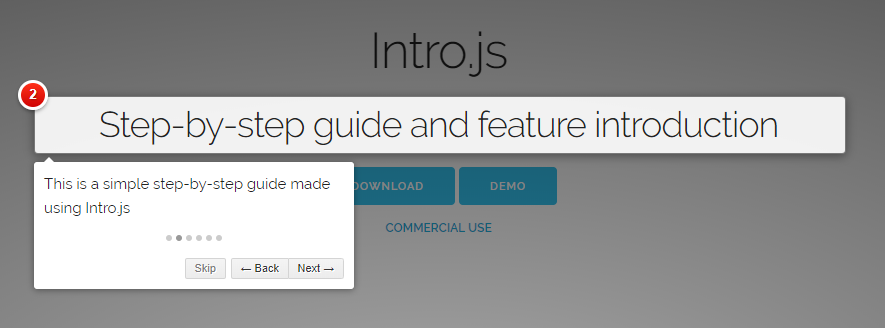
\includegraphics[width=\textwidth]{figures/intro_js_example.png}
        \caption{Anleitungs-Modus von Intro.js}\label{fig:intro_js_example}
\end{figure}

\subsubsection{``Offline-First''-Ansatz}
In jüngster Zeit ist es möglich mithilfe von Service-Worker \fixme{footnote?} und lokalen Speichermöglichkeiten im Browser Webseiten zu erstellen, die auch beim Aussetzenden Internetverbindungen mit minimalen Funktionen weiterhin funktionieren. So können etwa Änderungen welche an den Server geschickt werden müssen zwischengespeichert werden und sobald wieder eine Verbindung zum Internet besteht losgeschickt werden. Ein weiteres Beispiel ist das Anzeigen von Daten die vom letzten Besuch einer Seite stammen, wenn beim aktuellen Aufruf die Verbindung nicht stabil genug ist. Natürlich sollte ein Nutzer sowohl wenn er sich gerade im Offline-Modus befindet, als auch wenn wieder eine Verbindung besteht immer entsprechend informiert werden.
Vor allem auch in Kombination mit dem Ansatz die Bedienung einer Webseite für mobile Nutzer komfortabel zu gestalten ist es wichtig Verbindungsprobleme bereits mit einzuplanen und Nutzer nicht mit einer nicht-funktionalen Software alleine zu lassen.

\subsubsection{Intelligente Fehlerbehandlung}
Softwarefehler auf eine für den Benutzer angenehme Art und Weise zu behandeln und im Nachhinein detailliert zu analysieren ist bei traditioneller Software bereits ein nicht zu unterschätzendes Problem. Bei Webapplikationen kommt aber erschwerend hinzu, dass ein Teil der Logik nicht in einer Umgebung ausgeführt wird, welche man selbst kontrolliert (Browser auf Clientrechner). Umso wichtiger ist es, ein Konzept zu entwickeln um dort auftretende Fehler dennoch mit zu bekommen und auch genug Informationen zur künftigen Behebung dieser zu erhalten. Eine Lösung hierfür ist es, auftretende Fehler immer direkt zum Server zu schicken um sie vor Ort analysieren zu können --- wenn die eigene Infrastruktur dafür nicht ausreichend ausgebaut ist gibt es auch entsprechende Online-Dienste bei denen man ein solches Fehlerlog speichern kann. Zusätzlich dazu müssen auch Parameter für Serveranfragen mit höchster Vorsicht ausgewählt werden. Timeouts müssen lange genug sein, um eine Serverantwort nicht fälschlicherweise zu verwerfen und kurz genug um bei einem tatsächlichen Fehler die Applikation nicht zu träge wirken zu lassen. Zudem sollten im Fehlerfall erneute Versuche intelligent gestartet werden, also weder zu häufig um den Server nicht unnötig zu belasten als auch nicht zu selten um dennoch einen responsiven Eindruck zu vermitteln.

\subsubsection{Etablierte Authentifizierung}
Der \nameformat{\gls{crm}} besitzt zwar bereits ein integriertes Benutzersystem mit Rechteverwaltung, für die Portierung in das Internet sollte aber in Erwägung gezogen werden diese Rechteverwaltung mit einem oft genutzten, öffentlichen Protokoll wie OAuth oder ähnlichen Protokollen zu verbinden, um die Verbindung über HTTP und den Schutz der Authentisierungsdaten nicht mit einer selbst entwickelten, schlechter funktionierenden Lösung handhaben zu müssen.

\subsubsection{Caching}
Um Ressourcen zu sparen ist es von Vorteil, komplexe Berechnungen und lange dauernde Übertragungen nicht mehrmals auszuführen. Im Bereich des Webs gibt es mehrere Möglichkeiten, solche Daten temporär zu speichern: Die einfachste Form besteht darin, Antworten auf eingehende Anfragen auf dem Server und ebenso danach auf dem Client zu wieder zu verwenden. Wenn der Client selbst kein Caching unterstützt kann mit ``bedingten Anfragen'' dennoch der Cache des Servers genutzt werden --- es wird hierbei eine Anfrage an den Server geschickt und, sollte sich die Antwort im Vergleich zur letzten Anfrage nicht geändert haben, keine Daten, sondern nur ein entsprechender Hinweis an den Client zurück gesendet. Auch das HTTP-Protokoll unterstützt eingebaute Mechanismen (Cache-Header \fixme{footnote?}) um Caching beispielsweise über Cache-Proxies zu erleichtern. Bei allen Formen des Caching ist es jedoch kritisch, dass man die richtige Strategie zum Invalidieren der Daten auswählt um niemals mit zu stark veralteten Werten zu arbeiten, aber dennoch eine Effizienzsteigerung zu erreichen.

\subsubsection{Container}
Container-Technologien wie Docker oder Kubernetes helfen dabei, Abhängigkeiten der eigenen Software zu verwalten und auf jedem Entwicklungsrechner eine identische Umgebung zu schaffen. Auch für die Bereitstellung für Kunden ist es sehr viel einfacher einen bereits korrekt konfigurierten Container nur zu starten, anstatt eine komplette Umgebung auf einem Server einzurichten, vor allem wenn sich dieser Server bei externen Dienstleistern befindet. Da diese Konzepte bei der combit GmbH noch nicht eingesetzt werden ist es sinnvoll zu untersuchen, an welchen Stellen diese zu mehr Produktivität in Entwicklung und Verteilung der Software beitragen können.

\subsubsection{Serverless}
Unter ``Serverless'' versteht man das Konzept, dass als Firma keine eigenen Server für Kunden eingerichtet werden müssen, sondern stattdessen auf Lösungen von Drittherstellern (etwa AWS von Amazon oder \fixme{weiteres Beispiel}) gesetzt wird, auf denen die eigenen Serverkomponenten dann laufen. Firmenintern betreibt man also keine Server, ist also ``Serverless''. Der Vorteil von diesem Ansatz ist, dass die Verantwortung über die Serverhardware nicht selbst getragen werden muss und die Server durch die großen Kapazitäten der Hersteller je nach Belastung skaliert werden können. Im Gegenzug werden aber eigene Daten fremden Servern anvertraut, je nach Art und Sensibilität der Daten (Betriebsgeheimnisse, \gls{dsgvo} \fixme{footnote?}) kann dies nicht gewünscht sein. Ein solcher Ansatz muss daher gut abgewogen werden, bevor man ihn weiter verfolgt.

\subsubsection{Aktualisierungsstrategie}
Kontinuierliche Softwareupdates um Fehler auszubessern oder neue Features zu ergänzen sind heutzutage die Norm, es bedarf daher einer kompetenten Strategie um Veränderungen an Nutzer auszuliefern. Das Backend, auf dem auch die UI-Schicht gehostet wird, unterliegt allerdings nicht der Verantwortung der combit GmbH, weshalb Updates nicht direkt dort eingespielt werden können. Anstatt Updates für die Oberfläche an Updates des Backends zu koppeln sollte überlegt werden ob eine konfigurierbare Option angeboten werden kann um bei jedem Laden der Seite im Browser eine Updateprüfung auf einem zentralen combit-Server auszuführen. Dies bedingt allerdings, dass zwischen Oberfläche und Backend keinerlei Versionskopplung besteht. 

\subsubsection{Integration von bestehenden Ressourcen}
Auf der Webseite der combit GmbH gibt es bereits zahlreiche Ressourcen wie FAQ oder eine Knowledgebase zu verschiedenen Produkten. Um Nutzern diese Ressourcen präsenter anzubieten könnten diese direkt in die Oberfläche, etwa im Rahmen eines Hilfe-Modus, integriert werden.

\section{Anforderungen an den Entwicklungsprozess}
Neben den funktionalen Anforderungen ist es ebenso wichtig die richtigen Anforderungen für die Projektumgebung und -Entwicklung zu formulieren, um diesen Prozess möglichst effizient und skalierbar zu halten. Daher wird empfohlen folgende Technologien und Praktiken bei der Entwicklung des neuen Projektes zu nutzen:
\begin{itemize}
    \item{Tests}
    \item[] Alle in Kapitel~\ref{chap:technologies} vorgestellten UI-Frameworks enthalten bereits Lösungen um Tests auszuführen. Eine hohe Testabdeckung ist daher nicht nur nützlich um die Code zu erhalten und Regressionen zu erkennen sondern auch ohne hohe Kosten und Aufwand erreichbar.
    \item{Continuous Integration}
    \item[] Ein entsprechender TeamCity-Server von der Firma JetBrains ist firmenintern bereits vorhanden, daher sollten Tests von neuen Features immer auch auf diesem Server ausgeführt werden.
    \item{Codereviews}
    \item[] Pro Feature sollte auf einem gesonderten Branch gearbeitet und beim Zurückführen in den Masterbranch ein Review durch mindestens einen anderen Entwickler stattfinden um die Codequalität stets auf einem hohen Niveau zu halten. Auch für Reviews gibt es firmenintern bereits einen Upsource-Server (ebenfalls von der Firma JetBrains), welcher mit dem TeamCity-Server zusammen genutzt werden kann.
    \item{Git}
    \item[] Für bestehende Projekte wird bei der combit GmbH momentan SVN \fixme{footnote} als Versionskontrollsystem eingesetzt. Um die oben genannten Punkte besser umsetzen zu können wäre es von Vorteil neue Projekte zukünftig mit Git zu verwalten. Im Vergleich zu SVN ist das Erstellen und Integrieren eines Branches, welcher für Features und die damit verbundene CI und Reviews genutzt werden soll, bei Git simpler, da weniger Konflikte entstehen. \fixme{quelle}
\end{itemize}

\section{Hauptaugenmerk dieser Arbeit}
Eine komplette Umsetzung aller Anforderungen wäre im Rahmen dieser Thesis nicht zu bewältigen. Es gäbe zu viele Aspekte (geeignetes Hosting, eine sichere Authentifizierungsmethode, ein neuer Aktualisierungsmechanismus, etc.) die beachtet werden müssten, summiert reicht die Zeit nicht aus um Konzepte für all diese Aspekte in einer entsprechenden Qualität und Sorgfalt umzusetzen. 
Wie in diesem Kapitel bereits beschrieben kann die Oberfläche des \nameformat{\gls{crm}} in zwei Hauptbereiche unterteilt werden. Zum einen diejenigen UI-Elemente welche sich nicht mit den anzuzeigenden Daten ändern, in Abbildung~\ref{fig:crm_ui} zum Teil links und oberhalb der Detailansicht zu sehen (weitere Dialoge und Oberflächen werden kontextbasiert angezeigt), und zum anderen die Detail- und Listenansicht selbst. Die nicht datenabhängigen Elemente und Dialoge bestehen fast vollständig aus statischen Elementen mit teilweise speziellen Anforderungen welche bei der Umsetzung zwar zeitaufwändig wären, aber technisch kein interessantes Problem darstellen. Es wird im Weiteren daher nur die Oberfläche der Datenansichten (Detail- und Listenansicht) und die damit verbundenen Anforderungen betrachtet. 

Aus der Liste der funktionalen Anforderungen des \nameformat{\gls{crm}} also folgende Punkte:
\begin{itemize}
    \item{Automatisierte Erstellung}
    \item{Editier-Modus}
    \item{Individualisierung}
    \item{Suche / Filter / Sortierung}
\end{itemize}

Ein Vorteil von moderner, komponentenbasierter Webtechnologie (alle in Kapitel~\ref{chap:technologies} betrachteten Frameworks sind darauf ausgelegt) erlaubt es trotz der Trennung dieser UI-Bestandteile und der restlichen Oberfläche diese problemlos miteinander zu kombinieren. Es können sogar jeweils unterschiedliche Technologien für die jeweiligen Teile genutzt werden, durch das Transpilieren und herkömmliches HTML, CSS und JavaScript sind zur Laufzeit alle Umsetzungen miteinander kompatibel.
Bei dieser zweistufigen Umsetzung kann das Ergebnis dieser Arbeit außerdem bereits in der Webansicht der bestehenden Desktopapplikation angezeigt und als Alternative zu den nativen Oberflächen angeboten werden. So können Kunden dieses Feature bereits im Vorfeld testen und evaluieren und wichtiges Feedback für die weitere Entwicklung einbringen.
